\begin{figure}[ht]
    \centering
    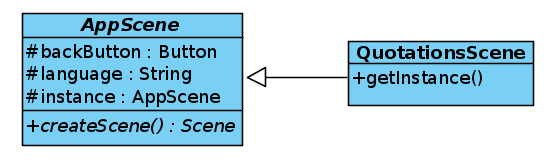
\includegraphics[scale=0.4]{img/classGUIBanqueAssurance.png}
    \caption{Ajout au diagramme de classe de la partie GUI de l'extension assurance}
    \label{fig1}
    \end{figure}

\paragraph{}Comme dit dans la partie client de l’extension assurance, les classes de logique et d’API ajoutées sont en commun avec la partie banque. Cependant la partie GUI ajoute une scene à l’application à savoir QuotationScene qui permet de gérer les demandes de devis. La classe AppScene est la même que celle des autres diagrammes, elle a juste été isolée ici pour une meilleur lisibilité.
